\section{Problem 1}

This problem will only address L type matching networks and work considering the load impedance higher than the source impedance ($R_L>R_S$). The second variant with $R_S>R_L$ will be addressed in the second problem.

\subsection{Designing the matching network}

The circuit without the matching network is a simple series association of a \texttt{Term} component representing the source and it has a impedance of $R_S=10 \Omega$ and another \texttt{Term} of impedance $R_L=100 \Omega$ representing the load. The desired resonance frequency must be $f_o = 10 GHz$.

First of all we simulate the circuit as it is, only concluding by the smith chart of figure \ref{fig:smith1} ($|S_{11}| \neq 0$) and the value of input impedance that there is no match between the terminal impedances. The input impedance was found with the ADS function \texttt{stoz} using the reflection coefficient $S_{11}$.

\begin{figure}[H] 
\centering
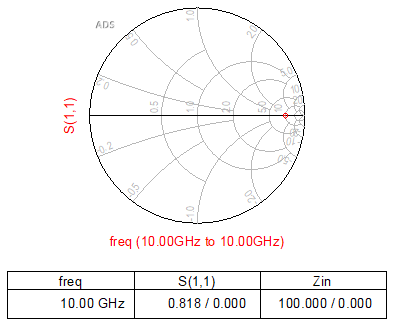
\includegraphics[width=8cm]{images/smith1.PNG}
\caption{Circuit $R_S=10 \Omega$ and $R_L=100 \Omega$ without matching network.}
\label{fig:smith1} 
\end{figure}

Since the input impedance seen from the source must be a lower value than the actual load impedance, the L network in figure \ref{graph:1} will promote a parallel to series impedance transformation in a way that the load impedance seen from the source point-of-view is $R_{in} = R_S$.


\begin{figure}[H]
\centering

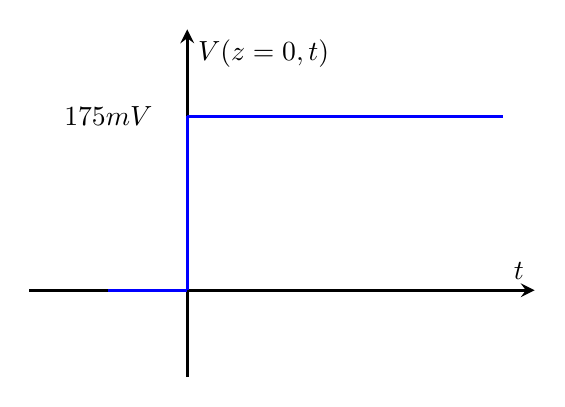
\begin{tikzpicture} 
\begin{axis}[very thick,
                     samples = 100,
                     ytick={-2,2},
                     xlabel = {$t$},
                     ylabel = {$V(z=0, t)$},
                     xmin = -1,
                     xmax = 2.2,
                     ymin = -0.5,
                     ymax = 1.5,
                     width=8cm,
                     height=6cm,
                     axis x line = middle,
                     axis y line = middle,
                     ticks = none]
                     
            \addplot[blue] coordinates {(-0.5,0) (0,0)};
            \addplot[blue] coordinates {(0,0) (0,1)};
            \addplot[blue] coordinates {(0,1) (2,1)};
            \node at (axis cs:-0.5,1){$175 mV$};
            
        \end{axis}
\end{tikzpicture}

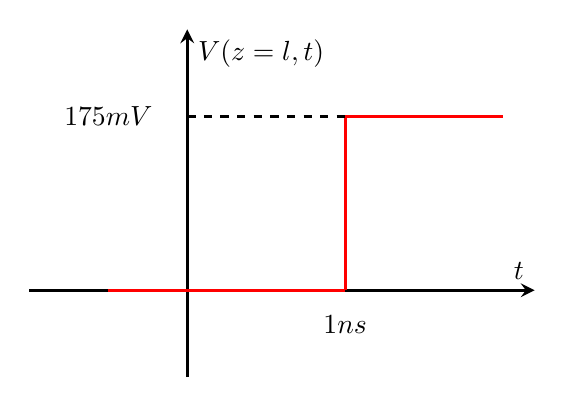
\begin{tikzpicture} 
\begin{axis}[very thick,
                     samples = 100,
                     ytick={-2,2},
                     xlabel = {$t$},
                     ylabel = {$V(z=l, t)$},
                     xmin = -1,
                     xmax = 2.2,
                     ymin = -0.5,
                     ymax = 1.5,
                     width=8cm,
                     height=6cm,
                     axis x line = middle,
                     axis y line = middle,
                     ticks = none]
                     
            \addplot[red] coordinates {(-0.5,0) (1,0)};
            \addplot[red] coordinates {(1,0) (1,1)};
            \addplot[red] coordinates {(1,1) (2,1)};
            \addplot[dashed] coordinates {(0,1) (1,1)};
            \node at (axis cs:-0.5,1){$175 mV$};
            \node at (axis cs:1,-0.2){$1ns$};
            
        \end{axis}
\end{tikzpicture}

\caption{First graph shows the voltage at the start of the line and the second shows the voltage at the end of the line. Source: own.}
\label{graph:1} 
\end{figure}

As seen in figure \ref{graph:1}(a), the impedance gain must reduce the value of the load impedance such in equation \ref{eq:1}.

\begin{equation} \label{eq:1}
    R_{in} = \frac{R_L}{1+Q_p^2}
\end{equation}

The quality factor for the parallel association is \ref{eq:2}:

\begin{equation} \label{eq:2}
    Q_p = \sqrt{\frac{R_L}{R_{in}}-1} = 3
\end{equation}

Since the inductance of the matching network is in parallel association with the load impedance, the parallel quality factor is also found as the relation between the resistance with the reactance, resulting in a expression for the network inductance \ref{eq:3}.

\begin{equation} \label{eq:3}
    Q_p = \frac{R_L}{L\omega_o} \Longrightarrow L = \frac{R_L}{Q_p\omega_o} = 0.53 \, nH
\end{equation}

To calculate the network capacitance we need to transform the parallel RL portion in a RL series association, transforming L in its series equivalent with equation \ref{eq:4}.

\begin{equation} \label{eq:4}
    L_s = \frac{L}{1+Qp^{-2}} = 477 \, pH
\end{equation}

The capacitance can be easily found by the resonance frequency expression \ref{eq:5}.

\begin{equation} \label{eq:5}
    \omega_o = \frac{1}{\sqrt{L_sC}} \Longrightarrow C = \frac{1}{L_s \omega^2} = 0.53 \, pF
\end{equation}

Despite finding a series inductance $L_s$, the network still be using the parallel L found before.

Using the same pattern of figure \ref{fig:smith1} we can produce a comparison with the results introducing the matching network found before, resulting in the figure \ref{fig:smith2}.

\begin{figure}[H] 
\centering
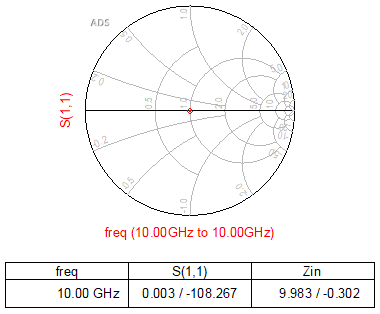
\includegraphics[width=8cm]{images/smith2.PNG}
\caption{Circuit $R_S=10 \Omega$ and $R_L=100 \Omega$ with matching network.}
\label{fig:smith2} 
\end{figure}

As we can see from the values of the reflection coefficient and the input impedance, they do not represent a perfect match due to rounding errors in the computation, but they are a good approximation for $|S_{11}| \approx 0$ and $Z_{in} \approx 10 \Omega$.

It is important to observe that the designed network has the capability of transform $R_L = 10 \Omega$ in $R_S = 100 \Omega$ just using the topology of figure \ref{graph:1} mirrored. The figure \ref{fig:smith3} illustrates the smith chart representing a match ($|S_{22}| \approx 0$) and the input impedance corresponding to the new source impedance $Z_{in} \approx 100 \Omega$.

\begin{figure}[H] 
\centering
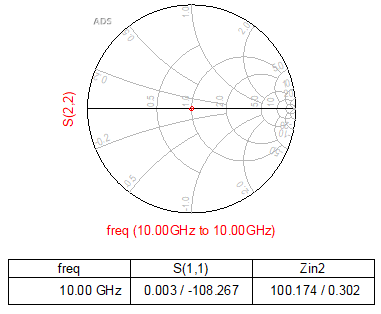
\includegraphics[width=8cm]{images/smith3.PNG}
\caption{Circuit $R_S=100 \Omega$ and $R_L=10 \Omega$ with matching network.}
\label{fig:smith3} 
\end{figure}

As a matter of comparison on future topics, we have designed a second L type matching network for a circuit with $R_S=20 \Omega$, $R_L=100 \Omega$ and $f_o = 10 GHz$ using the same methodology as before and same matching network topology (like in figure \ref{graph:1}), with quality factor $Q = 2$, inductance $L = 0.7958 \, nH$ and capacitance $C = 0.3979 \, pF$.

\subsection{Bandwidth}

To evaluate the different bandwidths from the circuits designed before we enumerated its terminals from 1 to 4. The circuit with a distinct $R_S=10 \Omega$ has a source terminal \#1 and a load terminal \#2. The circuit with a distinct $R_S=20 \Omega$ has a source terminal \#3 and a load terminal \#4.

In this way we can run a S-parameters simulation from 5 GHz up to 30 GHz and observe the -3dB and 90\% bandwidth of $|S_{21}|^2$ and $|S_{43}|^2$.

\subsubsection{-3dB bandwidth}

The -3dB bandwidth is calculated observing the value of $|S_{21}|^2$ and $|S_{43}|^2$ in a dB scale. As we can see in figure \ref{fig:bw1} with both curves overlapping, the second circuit with $R_S = 20 \Omega$ has a higher bandwidth, once the quality factor is lower than the other circuit and the bandwidth obey the relation $\Delta\omega_{-3dB} = \omega_o / Q = 3.33 GHz \; \text{for} \; Q=3 \; \text{and} \; 5 GHz \; \text{for} \; Q=2 $.

\begin{figure}[H] 
\centering
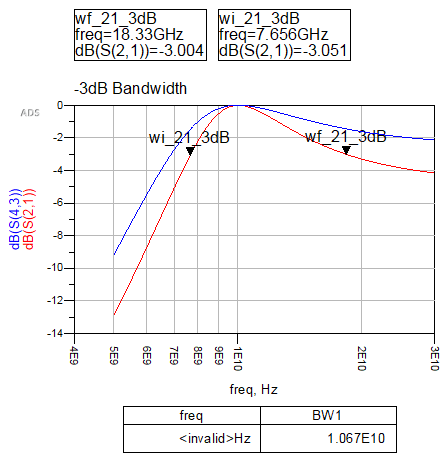
\includegraphics[width=8cm]{images/BW1.PNG}
\caption{-3dB bandwidth for $|S_{21}|^2$ and $|S_{43}|^2$.}
\label{fig:bw1} 
\end{figure}

The value for the second circuit -3dB bandwidth was not determined since $|S_{43}|^2$ does not cross the -3dB value a second time.

\subsubsection{90\% bandwidth}

The 90\% bandwidth tends to be narrower than the -3dB, representing only a third of the previous value ($\Delta\omega_{90\%} = \Delta\omega_{-3dB}/3 = 1.11 GHz \; \text{for} \; Q=3 \; \text{and} \; 1.66 GHz \; \text{for} \; Q=2 $). In this case, the values of $|S_{21}|^2$ and $|S_{43}|^2$ are better seen in a linear scale since the limits of the 90\%bandwidth will be 0.9. The figure \ref{fig:bw2} show the results.

\begin{figure}[H] 
\centering
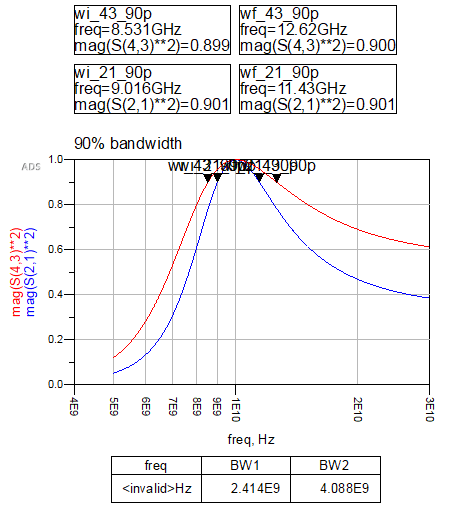
\includegraphics[width=8cm]{images/BW2.PNG}
\caption{90\% bandwidth for $|S_{21}|^2$ and $|S_{43}|^2$.}
\label{fig:bw2} 
\end{figure}

The results allow us to define the bandwidths for both circuits. As mentioned in the previous topic, the bandwidth for the circuit with $R_S = 20 \Omega$ still higher than the other circuit as expected.

\subsubsection{Comparison}

First comparing the -3dB theoretical bandwidth of 3.33 GHz with the value obtained in practice 10 GHz it is clearly seen a large discrepancy. This is explained once a additional source resistance is added to the RLC circuit, with both load and source resistance equal, thus resulting in two more times dissipated energy and halving the quality factor, resulting in the double of bandwidth in practice. The remaining discrepancy is explained once the quality factor definition relies on a RLC circuit, and when we associate the resistance of both source and load in different ends of the circuit with the matching network, we achieve a perfect RLC circuit no more . So the previous analysis for the quality factor only serves as approximation for what we can expect from this kind of circuit.

Now comparing the -3dB bandwidth of the circuit 1 in figure \ref{fig:bw1} with its equivalent in the 90\% bandwidth in figure \ref{fig:bw2} we observe a scaling difference of 4.42 times, although it was expected a relation of 3. This behaviour is reminiscent of the problem above.

